\documentclass{article}

\usepackage{Sweave}
\begin{document}
\Sconcordance{concordance:aula4.tex:aula4.rnw:%
1 2 1 1 0 5 1 1 2 1 0 1 1 1 6 4 0 1 4 2 0 1 1 1 3 2 1 1 5 3 0 1 1 1 2 1 %
1 1 2 1 1 1 2 1 1 1 4 2 0 1 1 1 2 1 1 1 4 2 0 1 11 10 0 1 2 3 1 4 0 1 2 %
2 1}


\section{Distribuicao bimodal}


\begin{Schunk}
\begin{Sinput}
> library("rgl")
> rm(list=ls())
> fnormal1var <- function(x,m,r)
+ {
+   y <- (1/(sqrt(2*pi*r*r)))*exp(-0.5*((x-m)/(r))^2)
+   return(y)
+ }
> ###########################
> 
> c1 <- matrix(rnorm(100, mean = 2, sd = 0.4),ncol=2)
> c2 <- matrix(rnorm(100, mean = 4, sd = 0.4),ncol=2)
> plot(c1[,1], c1[,2], col='red', type='p', xlim=c(0,6), ylim=c(0,6),xlab='x_1',ylab='x_2')
> par(new=T)
> plot(c2[,1], c2[,2], col='blue', type='p', xlim=c(0,6), ylim=c(0,6),xlab='',ylab='')
> ############################
> 
> ##C1-
> m11 <- mean(c1[,1])
> s11 <- sd(c1[,1])
> m12 <- mean(c1[,2])
> s12 <- sd(c1[,2])
> m21 <- mean(c2[,1])
> s21 <- sd(c2[,1])
> m22 <- mean(c2[,2])
> s22 <- sd(c2[,2])
> ############################
> 
> seqi <- seq(0,6,0.1)
> seqj <- seq(0,6,0.1)
> M1 <- matrix(0,nrow =length(seqi),ncol=length(seqj))
> M2 <- matrix(0,nrow =length(seqi),ncol=length(seqj))
> ############################
> 
> ci <- 0
> for (i in seqi)
+ {
+   cj <- 0
+   ci<- ci + 1
+   for (j in seqj)
+   {
+     cj <- cj + 1
+     M1[ci,cj]<-fnormal1var(i,m11,s11)*fnormal1var(j,m12,s12)
+     M2[ci,cj]<-fnormal1var(i,m21,s21)*fnormal1var(j,m22,s22)
+   }
+ }
> classx<-0.5*(M1 >= M2) #limiar
> persp3d(seqi,seqj,M1,col='red',clim=c(0,2),colkey=F)
> persp3d(seqi,seqj,M2,col='blue',clim=c(0,2),add=T,colkey=F)
> persp3d(seqi,seqj,classx,col='black',clim=c(0,2),add=T,colkey=F)
\end{Sinput}
\end{Schunk}
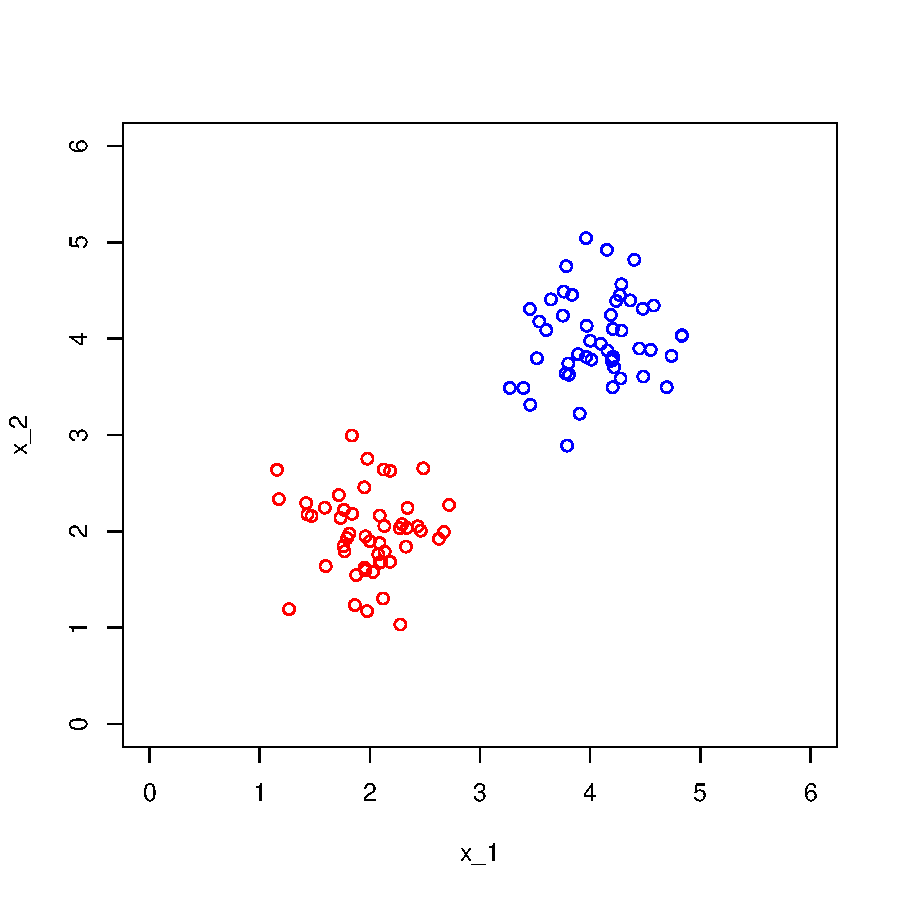
\includegraphics{aula4-001}


\end{document}
